\section{Minimierung mittels des
Table-Filling-Algorithmus}

\subsection{Der Algorithmus}
Der Table-Filling Algorithmus\cite{minimization1,minimization2,minimization3} ist abgeleitet
 vom Äquivalenzsatz von Myhill und Nerode. 

Es wird eine Matrix benötigt, in der in den Zeilen und Spalten alle Zustände des
Automaten vorhanden sind.

Die Grundidee ist, dass in dieser Matrix alle Paare von Zuständen markiert
werden die nicht äquivalent sind.

{\bf Formal: \\}
Seien P und Q zwei Zustände, $\omega$ ein Satz (eine Folge von Terminale), und X
= $\delta$(P,$\omega$) und Y = $\delta$(P,$\omega$) die nachfolgende Zustände von P und Q mit eingabe
$\omega$ .

P und Q sind zwei nicht-äquivalente Zustände, wenn ein Zustand vom
Zustandspaar (X,Y) ein akzeptierender Zustand und der Andere ein
nichtakzeptierender Zustand ist.

Falls für den Paar (P,Q) nicht entschieden werden kann ob die zwei Zustände
äquivalent sind oder nicht, werden die Zustände zu die Abhängigkeiten
(dependencies) der Nachfolgenden Zustände (X,Y) hinzugefügt. (P,Q) werden
später die Eigenschaft von (X,Y) haben.

%Workaround um Probleme mit UTF-8 und listings zu beheben
\lstset{language=C, basicstyle=\footnotesize}
\lstset{literate=%
{Ö}{{\"O}}1
{Ä}{{\"A}}1
{Ü}{{\"U}}1
{ß}{{\ss}}2
{ü}{{\"u}}1
{ä}{{\"a}}1
{ö}{{\"o}}1
}
\begin{lstlisting}[float=h!, frame=tb, captionpos=b,
caption={Table-Filling-Algorithmus : Pseudocode}, label=list:TablefillingCode]
1.Initialisiere alle Paare in der Matrix als nicht-markiert,
 und ohne "dependencies".
2.Markiere alle Paare von akzeptierenden Zuständen und 
nicht-akzeptierenden Zuständen als nicht-äquvalent.
3.Für alle nicht markierte Paare (P,Q) und jedes Eingabesymbol a:
	Sei X = delta(P,a), Y = delta(Q,a).
	Falls (X,Y) nicht markiert, 
		füge (P,Q) zu den dependencies von (X,Y) hinzu,
	Sonst markiere (P,Q), und markiere alle dependencies von (P,Q).
	
\end{lstlisting}

\subsection{Implementierung}
\cite{minimization4,minimization5}
Um diesen Algorithmus zu impelementieren, wurde eine neue Klasse
\textit{TableFillingMinimizer} erstellt. Diese Klasse bietet die benötigten
Methoden um einen endlichen Zustandsautomat zu minimieren.

\begin{figure}[h]
  \begin{center}
  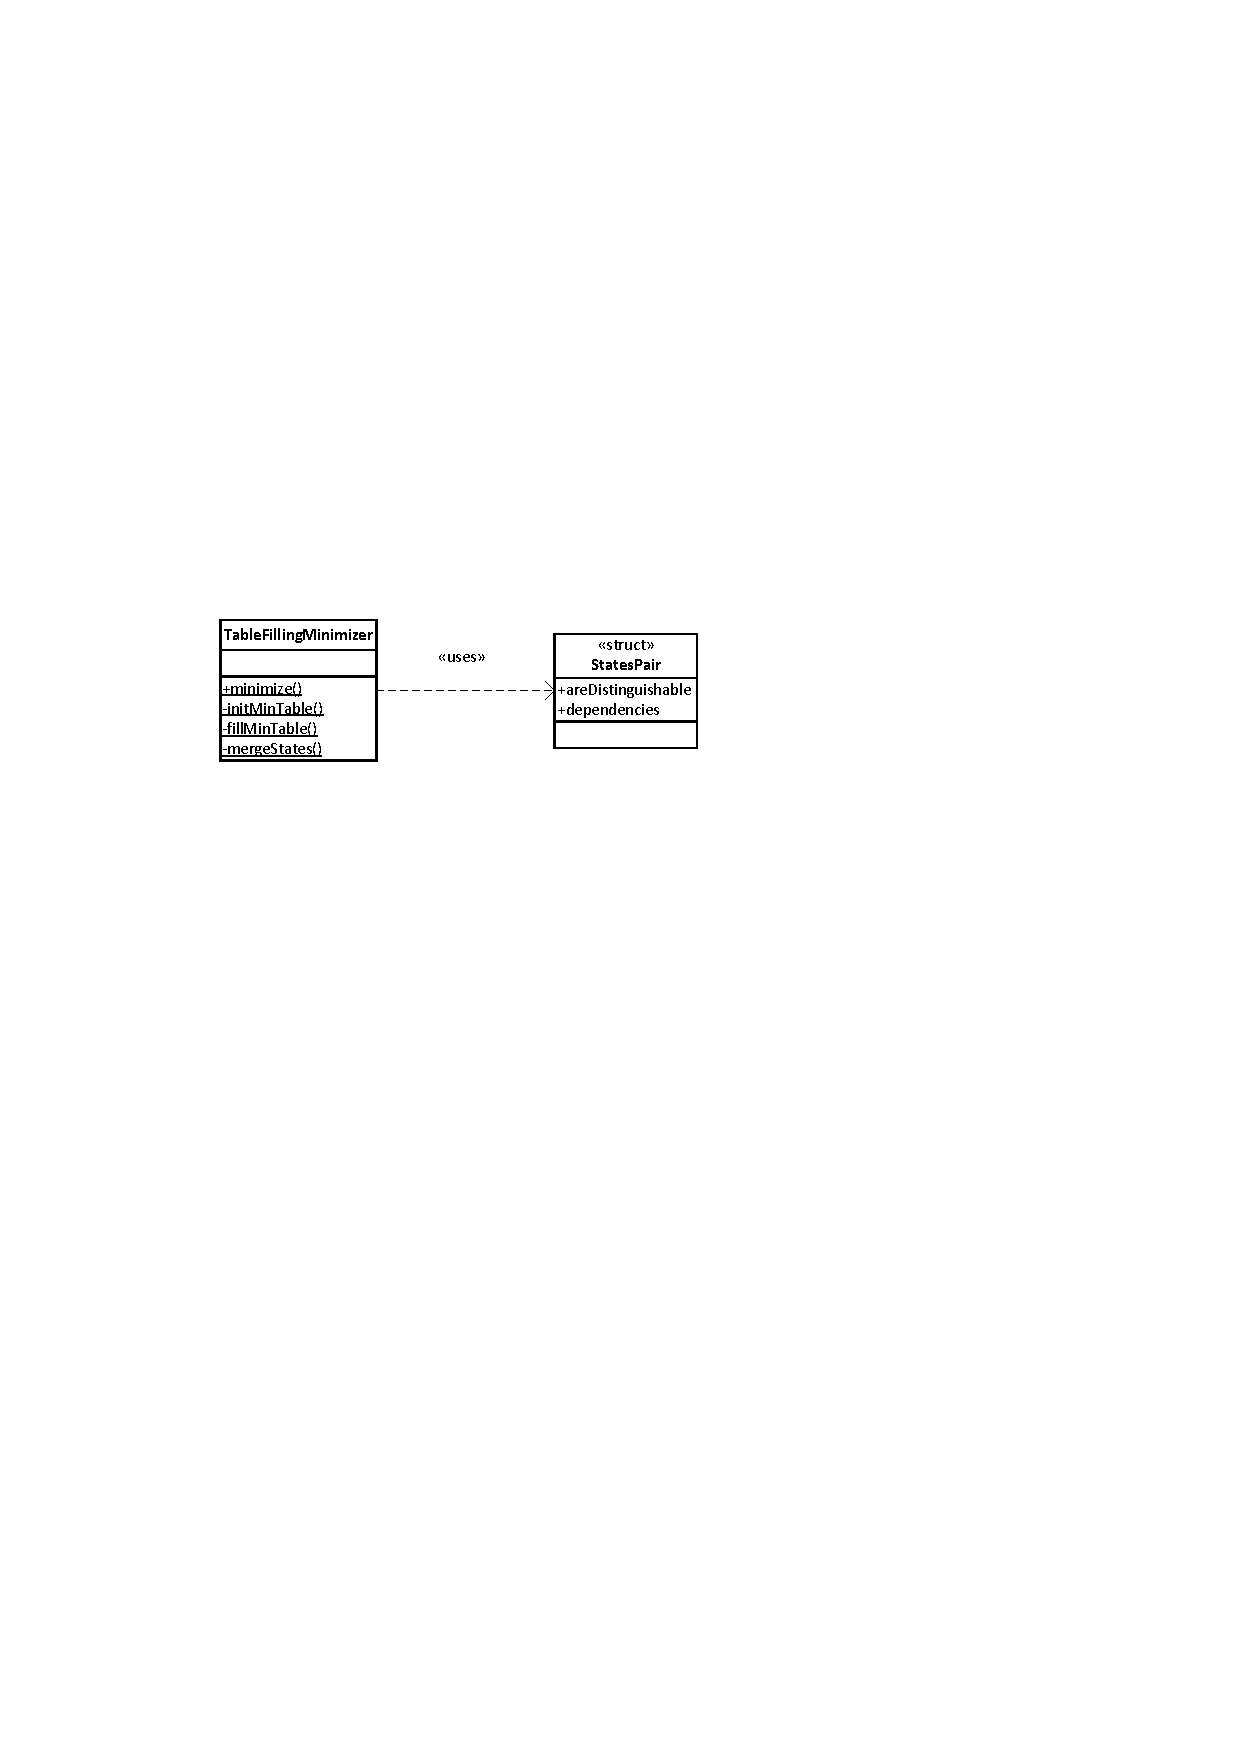
\includegraphics{objectsToInclude/TableFillingMinimizer.pdf}
  \caption{UML Diagramm zu \textit{TableFillingMinimizer}}
  \label{fig:UMLminTable}
  \end{center}
\end{figure}

Die verwendete Matrix in diesem Algorithmus ist eine Matrix von
\textit{StatesPair}, wobei jedes \textit{StatesPair} eine Struktur ist in der
gespeichert wird ob ein Paar nicht-äquivalent ist, und eine Liste mit den
Abhängigkeiten dieses Paares.